
%(BEGIN_QUESTION)
% Copyright 2015, Tony R. Kuphaldt, released under the Creative Commons Attribution License (v 1.0)
% This means you may do almost anything with this work of mine, so long as you give me proper credit

Anta at en reguleringsventil brukes til å strupe væske inn i et reservoar som deretter tømmes ved selvfall til en prosess. Et nivåreguleringssystem (ikke vist) styrer reguleringsventilen etter behov for å holde konstant væskenivå i reservoaret, over et typisk strømningsområde på 0 til 100 gallon per minutt:

$$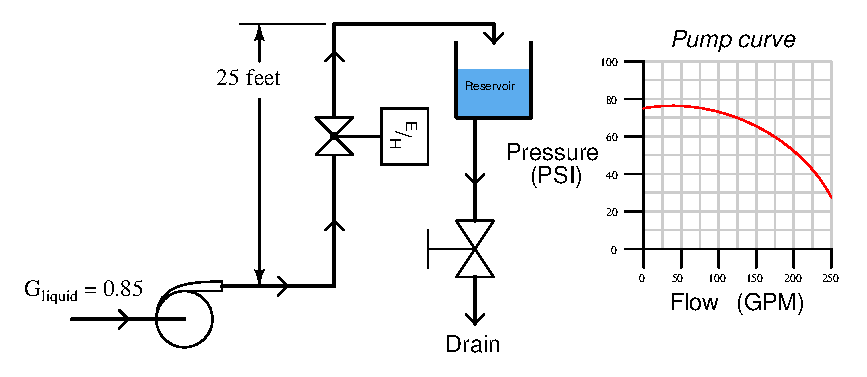
\includegraphics[width=15.5cm]{i01180x02.eps}$$

Basert på informasjonen i den enkle PFD-en og pumpekurven, avgjør om en reguleringsventil med lineær karakteristikk faktisk vil opptre lineært (dvs. ha lineær {\it installert} karakteristikk) i denne prosessen. Forklar resonnementet ditt i detalj.

\vskip 10pt

Avgjør deretter det samme for følgende prosess, der reguleringsventilen struper væske gjennom en spraydyse over samme typiske strømningsområde på 0 til 100 GPM:

$$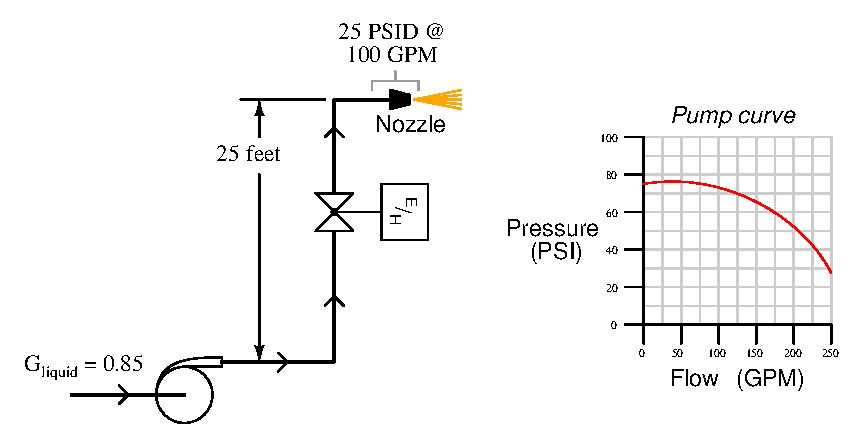
\includegraphics[width=15.5cm]{i01180x01.eps}$$

\vskip 20pt \vbox{\hrule \hbox{\strut \vrule{} {\bf Forslag til sokratisk diskusjon} \vrule} \hrule}

\begin{itemize}
\item{} Forklar generelt hvor og hvorfor vi kan trenge en ``karakterisert'' reguleringsventil for å oppnå lineær strømningsregulering i en prosess.
\item{} Vil reguleringsventiler med samme $C_v$-verdi fungere like godt i begge scenarier? Forklar hvorfor eller hvorfor ikke. Hvis ulike $C_v$-verdier er nødvendige, hvilket scenario krever en ventil med høyere $C_v$?
\item{} Det er generelt dårlig praksis å ``dead-heade'' en sentrifugalpumpe (dvs. å blokkere utløpslinjen fullstendig mens pumpen går, slik denne reguleringsventilen gjør når den er stengt). Identifiser flere måter å løse dette problemet på, slik at pumpen aldri kan ``dead-heade'' uansett hvilken stilling reguleringsventilen står i.
\end{itemize}

\underbar{file i01180}
%(END_QUESTION)





%(BEGIN_ANSWER)

{\it Hint: varierer trykkfallet over reguleringsventilen vesentlig med gjennomstrømningen?}
 
%(END_ANSWER)





%(BEGIN_NOTES)

Det første prosesseksemplet (innstrømning til et åpent reservoar) vil gi lineær installert karakteristikk, fordi trykkfallet over reguleringsventilen vil være nesten konstant over hele strømningsområdet (0-100 GPM).  Pumpekurven viser at utløpstrykket holder seg relativt flatt (omtrent 70 til 77 PSI) i forventet område, og siden den statiske løftehøyden (25 fot ved spesifikk vekt 0.85) er konstant og utløpstrykket i røret er 0 (atmosfærisk), betyr dette at reguleringsventilen får et relativt konstant trykkfall:

$$\Delta P = 70 - \left(25 \hbox{ ft liquid} \over 1 \right)  \left(12 \hbox{ in} \over 1 \hbox{ ft}\right)  \left(1 \hbox{ PSI} \over 27.68 \hbox{ "WC}\right)  \left(0.85 \hbox{ "WC} \over 1 \hbox{ " liquid}\right) = 60.79 \hbox{ PSID minimum}$$

$$\Delta P = 77 - \left(25 \hbox{ ft liquid} \over 1 \right)  \left(12 \hbox{ in} \over 1 \hbox{ ft}\right)  \left(1 \hbox{ PSI} \over 27.68 \hbox{ "WC}\right)  \left(0.85 \hbox{ "WC} \over 1 \hbox{ " liquid}\right) = 67.79 \hbox{ PSID maximum}$$

En variasjon på 7 PSI er bare litt mer enn 10\% av grunnleggende trykkfall over ventilen.  Tegner vi denne ``lastlinjen'' oppå et sett karakteristikkurver for en iboende lineær ventil, får vi skjæringspunkter som er nesten jevnt fordelt:

$$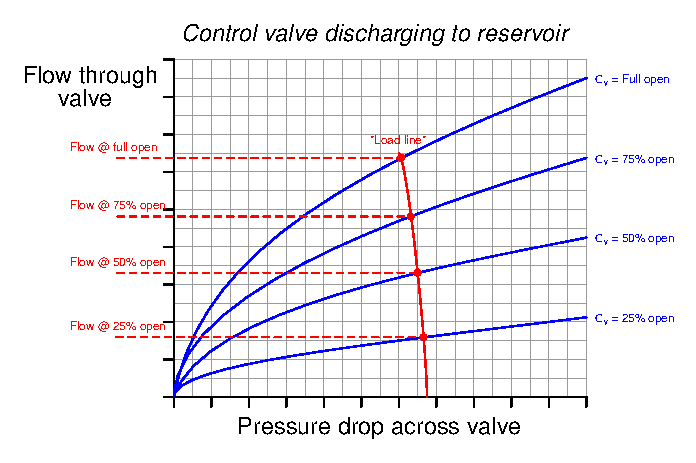
\includegraphics[width=15.5cm]{i01180x03.eps}$$

\vskip 10pt

\filbreak

I det andre prosesseksemplet vil imidlertid innkobling av en spraydyse i rørsystemet introdusere et variabelt trykkfall på 0 til 25 PSID over samme strømningsområde.  Det betyr at ventilens trykkfall blir 25 PSID lavere ved full gjennomstrømning (100 GPM), mens det er som før ved null gjennomstrømning.  Denne større, gjennomstrømningsavhengige variasjonen i tilgjengelig trykk vil forvrenge ventilens installerte karakteristikk, og krever dermed likprosentlig ventilkarakteristikk i stedet for iboende lineær karakteristikk.

Denne større variasjonen gir en lastlinje med skarpere krumming, og dermed et sett skjæringspunkter som {\it ikke} er jevnt fordelt:

$$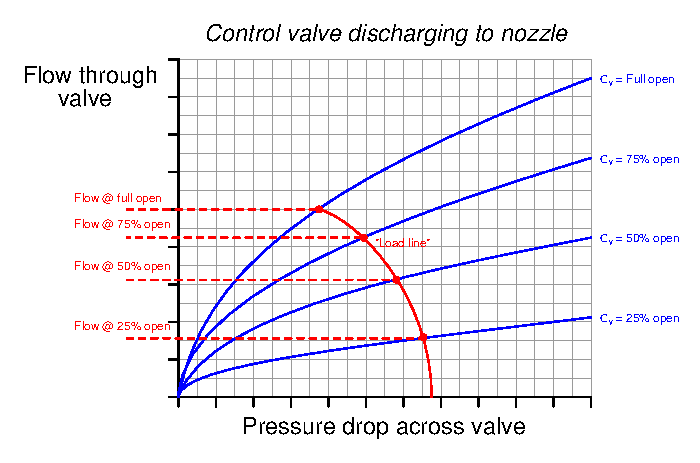
\includegraphics[width=15.5cm]{i01180x04.eps}$$

For øvrig forutsetter dette kurvesettet bruk av en større reguleringsventil, for å oppnå samme maksimale gjennomstrømning med mindre tilgjengelig trykk.

%INDEX% Sluttkontrollelementer, pumpe: trykk/flow-kurve
%INDEX% Sluttkontrollelementer, ventil: karakterisering

%(END_NOTES)
